%%=============================================================================
%% Inleiding
%%=============================================================================

\chapter{\IfLanguageName{dutch}{Inleiding}{Introduction}}%
\label{ch:inleiding}

De Belgische wijnbouwsector heeft de afgelopen twintig jaar een opmerkelijke groei doorgemaakt.  Twintig jaar geleden was er nauwelijks sprake van wijnbouw, maar de sector is de laatste jaren uitgegroeid tot een productieve pijler binnen onze landbouw. Volgens \textcite{FODEconomie2024} werd er in 2023 meer dan 3,4 miljoen liter wijn geproduceerd, en die groei zet zich voort. Ten opzichte van het voorgaande jaar steeg de productie met bijna dertien procent, terwijl het aantal hectaren met elf procent toenam. 

Vanwege deze opmars krijgt de sector aandacht binnen het \textit{Flanders AI Research Programme} (FAIR). FAIR is een consortium van onderzoeksgroepen aan Vlaamse universiteiten en onderzoekscentra, gericht op AI-onderzoek in diverse Vlaamse sectoren. Het Instituut voor Landbouw-, Visserij- en Voedingsonderzoek (ILVO) is een van deze centra. Binnen het programma wordt onderzocht hoe AI kan bijdragen aan innovatie en duurzaamheid.

ILVO en UAntwerpen werken samen aan een AI-toepassing die wordt ingezet in wijngaarden. Hiermee kunnen kleine landbouwrobots autonoom taken uitvoeren, zoals het monitoren van de druivenkwaliteit. Hiervoor wordt een reinforcement learning (RL)-algoritme ontwikkeld en geïmplementeerd op ILVO's Treebot. \begin{figure}
    \centering
    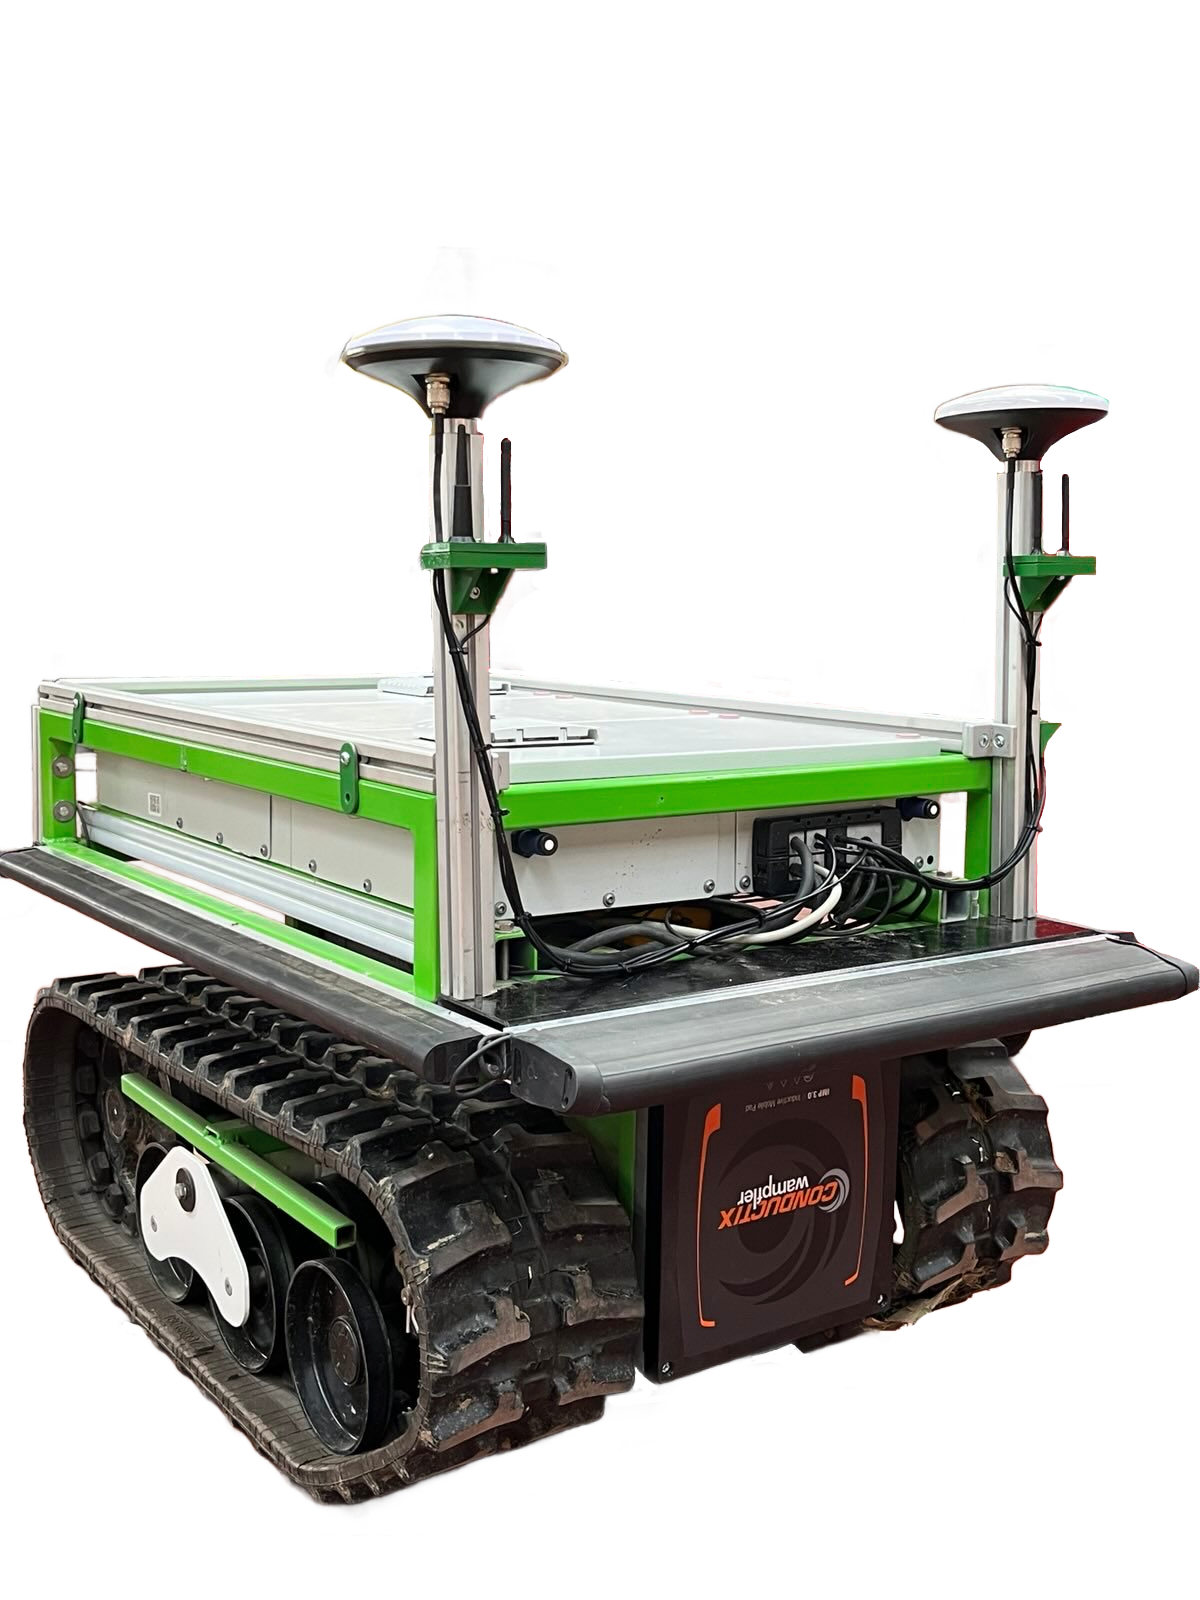
\includegraphics[width=0.5\textwidth]{treebot.png}
    \caption[Treebot ILVO.]{\label{fig:treebot}Treebot ILVO.}
\end{figure}

De robot beschikt over een arm en sensoren om druiven te inspecteren. Om een taak autonoom uit te voeren zijn momenteel drie controlesystemen nodig: navigatiecontrole, actuatorcontrole en taakcontrole. Het RL-algoritme moet deze controllers samenvoegen tot één geïntegreerde controller zodat de robot zelfstandig beslissingen kan nemen, afhankelijk van de situatie.

Om correcte beslissingen te nemen, heeft het RL-algoritme duidelijke omgevingsinformatie nodig. Dit betekent dat de robot druivenranken en -trossen rondom zich moet herkennen. Op Treebot wordt hiervoor een cameraplatform gemonteerd. De bachelorproef draagt bij aan de interpretatie van deze beelden en de vegetatie door semantische segmentatie toe te passen.

Het trainen van een dergelijk model is niet vanzelfsprekend, aangezien een grote hoeveelheid gelabelde data nodig is. Dit vormt een uitdaging voor semantische segmentatie in elke sector, maar in een wijngaardcontext is dit nog lastiger. De planten hebben een complexe, organische structuur met overlappende bladeren en variabele vormen, wat het labelen op pixelniveau bijzonder uitdagend maakt. Het correct onderscheiden van druivenranken en -trossen ten opzichte van de achtergrond vraagt daarom meer precisie en inspanning dan bij objecten met duidelijke contouren. Binnen deze bachelorproef wordt onderzocht in welke mate synthetische data kan bijdragen aan het opvangen van dit tekort en het efficiënter maken van het trainingsproces.

\section{\IfLanguageName{dutch}{Probleemstelling}{Problem Statement}}%
\label{sec:probleemstelling}

Treebot, de landbouwrobot van ILVO, heeft visuele waarneming nodig om zelfstandig in wijngaarden te werken. Om een gepaste actie te kiezen, moet de robot kunnen zien waar de druivenranken en -trossen zich bevinden. Machinevisie kan dit mogelijk maken, specifiek in de vorm van semantische segmentatie. Hierdoor kan hij de gewassen herkennen en onderscheiden van de achtergrond.

Het semantische segmentatiemodel moet in realtime de druivenranken en -trossen kunnen segmenteren. De implementatie van dergelijke modellen op edge devices, zoals kleine landbouwrobots, vormt een uitdaging vanwege beperkte rekenkracht en geheugen. Daarnaast presteren deze modellen vaak minder goed in een landbouwcontext, omdat hun architectuur niet is afgestemd op de complexiteit en variabiliteit van natuurlijke omgevingen. Het grootste struikelblok blijft echter het beperkte aantal beschikbare en gelabelde datasets. Het annoteren van wijngaardbeelden is namelijk een zeer tijdrovend en arbeidsintensief proces. Dit bemoeilijkt de training en generalisatie van een model aanzienlijk.

\section{\IfLanguageName{dutch}{Onderzoeksvraag}{Research question}}%
\label{sec:onderzoeksvraag}

Bovenstaande knelpunten leiden tot de hoofdonderzoeksvraag van deze bachelorproef: \emph{'Hoe kan een deep learning-model worden toegepast voor realtime segmentatie van druivenranken en -trossen in wijngaarden, en hoe draagt synthetische data bij aan de generalisatie?'} 

Om bovenstaande onderzoeksvraag te beantwoorden, worden verschillende deelaspecten onderzocht. Deze staan geformuleerd in de volgende deelvragen:

\begin{itemize}
    \setlength{\itemsep}{0pt}
    \setlength{\parskip}{0pt}
    % \item Wat zijn de natuurlijke en visuele kenmerken van een wijngaard?
    \item Welke uitdagingen ondervinden segmentatiemodellen bij toepassing in de landbouw?
    \item Welke modellen zijn geschikt voor druivenranken en -trossen?
    \item Op welke manier dient synthetische data samengesteld te worden om het segmentatiemodel beter te trainen?
    \item Hoe kan modeloptimalisatie plaatsvinden om segmentatie in realtime op edge devices mogelijk te maken?
\end{itemize}

Samen vormen ze de basis voor het verdere verloop van dit werk.

\section{\IfLanguageName{dutch}{Onderzoeksdoelstelling}{Research objective}}%
\label{sec:onderzoeksdoelstelling}

Het eindresultaat is een proof-of-concept van het segmentatiemodel, gericht op het herkennen van gewassen in wijngaarden. Daarbij is rekening gehouden met de hardwarebeperkingen van de landbouwrobot. De visuele invoer waarop het model werd getraind, bestaat grotendeels uit synthetische beelden. De modelprestaties en evaluatieresultaten in dit onderzoek bepalen in welke mate synthetische data bijdraagt aan een verbeterde generalisatie van het model. Zo wordt duidelijk of synthetische data bruikbaar is bij een tekort aan gelabelde wijngaarddata.

\section{\IfLanguageName{dutch}{Opzet van deze bachelorproef}{Structure of this bachelor thesis}}%
\label{sec:opzet-bachelorproef}

De bachelorproef is als volgt opgebouwd:

In Hoofdstuk~\ref{ch:stand-van-zaken} wordt een overzicht gegeven van de stand van zaken binnen het onderzoeksdomein, op basis van een literatuurstudie.

In Hoofdstuk~\ref{ch:methodologie} worden de methodologie en onderzoekstechnieken besproken, samen met een antwoord op de eerste twee deelvragen.

% TODO: Vul hier aan voor je eigen hoofstukken, één of twee zinnen per hoofdstuk

In Hoofdstuk~\ref{ch:synthetische-data} wordt de synthetische data verzameld door gesimuleerde afbeeldingen te genereren. De labels worden hierbij automatisch bekomen.

In Hoofdstuk~\ref{ch:proof-of-concept} wordt het semantische segmentatiemodel uitgewerkt. Eerst volgt een evaluatie na training met reële data, daarna een tweede evaluatie met toevoeging van synthetische data.

In Hoofdstuk~\ref{ch:conclusie}, tenslotte, wordt de conclusie gegeven en een antwoord geformuleerd op de onderzoeksvragen. Daarbij wordt ook een aanzet gegeven voor toekomstig onderzoek binnen dit domein.